% Source of paper/manuscript.tex. Every result is a value marker (backslash-val with an id) that scripts/render_manuscript.py replaces with
% the string docs/summary_values.json prints for it; the manuscript holds no hand-typed result.
% Drafting class: IEEEtran [journal,9pt] stands in for IEEE_lsens.cls (results/gates/G1_environment_rerun2.json);
% swap in IEEE_lsens.cls from the IEEE Sensors Letters template before submission and check the 4-page limit.
\documentclass[journal,9pt]{IEEEtran}
\usepackage{amsmath,amssymb}
\usepackage{graphicx}
\usepackage{booktabs}
\usepackage{cite}
\usepackage[hidelinks]{hyperref}

\begin{document}

\title{How Much of Wearable Activity-Recognition Accuracy Is the Network? A Pre-Registered Variance Decomposition
Under Person-Disjoint Evaluation}

\author{[Authors and affiliations to be added by the authors]}

\maketitle

\begin{abstract}
Wearable inertial activity-recognition systems are compared by their macro-F1 on people unseen in training, but how
much of that figure reflects the network and how much the people who happen to be tested has not been measured. We
decompose the variance of stored runs of one fixed person-disjoint protocol (WHAR Arena v1) with a linear mixed model
whose confirmatory test was pre-registered. On \val{H1.datasets} held-out datasets (\val{H1.runs} runs of four
networks with three training seeds), the group of test subjects accounts for \val{H1.pi_P}\,\% of the within-dataset
variance, \val{H1.R} times (97.5\,\% interval \val{H1.R_lo}--\val{H1.R_hi}) the variance of all network-related terms
together, and the pre-registered criterion was met. The ordering also holds with a metric free of per-split
ceilings and on the development datasets, where its interval includes 1 for that metric. It reverses across the
benchmark's 17 heterogeneous published architectures, where the network dominates. Between comparable networks, the
subjects a wearable study records bound what an accuracy difference can show.
\end{abstract}

\begin{IEEEkeywords}
Wearable sensors, inertial sensors, human activity recognition, person-disjoint evaluation, variance components,
mixed models.
\end{IEEEkeywords}

\section{Introduction}
Wearable inertial sensing systems for human activity recognition (HAR) are designed and chosen on one number:
macro-F1 on subjects held out from training~\cite{bulling2014tutorial}. Evaluating on unseen people removes the
optimism of random cross-validation~\cite{hammerla2015lets}, and how people are partitioned between training and test
data changes the reported accuracy~\cite{lockhart2014limitations}. People move differently~\cite{qian2021latent} and
devices sense differently~\cite{stisen2015smart}, so a test set of a few subjects carries its own variation. WHAR
Arena~\cite{burzer2026arena} fixed one person-disjoint protocol across 30 datasets and found the state of the art
distributed over architectures rather than held by one; it reports one training run per split, so it cannot separate
the effect of who is tested from the training seed. Machine-learning benchmarks are known to depend on such sources of
variation~\cite{bouthillier2021accounting}, but their sizes in wearable HAR are unknown.

This letter measures them. Under one fixed protocol it decomposes the variance of macro-F1 into the group of test
subjects, the network, their interactions and the training seed; it tests the ordering of these terms with a
pre-registered analysis on held-out datasets; it checks the result with a ceiling-free metric, development data and
the benchmark's independent architectures; and it reports, as exploratory, which design choices and which sensing
properties of a dataset go with large accuracy differences.

\section{Methods}
\subsection{Protocol and stored runs}
All runs follow WHAR Arena v1 with its paper-era code~\cite{burzer2026arena,burzer2025whar}: 3-s windows with 50\,\%
overlap at the native sampling rate; $k=10$ subject groups, each split testing on one group
(\val{subjects_per_split.min} to \val{subjects_per_split.max} subjects) that never appears in training or validation;
validation from 20\,\% of the training subjects' windows; a z-score fitted on the training split; macro-F1 over all
classes, with classes absent from a test split counted as 0. No network was trained for this letter: we analyse stored
runs and their checkpoints. Three sets enter (Table~\ref{tab:vc}): S1, ten networks that share one skeleton and differ
in single components (with and without temporal memory, e.g.\ S4D~\cite{gu2022efficiently,gu2022parameterization} and
Mamba~\cite{gu2023mamba}, or window statistics), on ten development datasets with three seeds; S2, four of these
networks on eight datasets never used for this question, with three seeds; S3, the benchmark's 17 published models
(deep networks such as DeepConvLSTM~\cite{ordonez2016deep,hammerla2016deep}, and Random Forest~\cite{breiman2001random},
SVM and k-NN on tsfresh features~\cite{christ2018tsfresh}) re-run with the same code on four datasets, one run per
split. A pre-registered inclusion rule removed datasets whose stored runs disagree on split sizes, because their split
indices do not name the same subjects across runs (one dataset each in S1 and S2).

\subsection{Variance model and pre-registered test}
For run $(m,d,s,r)$ of network $m$ on split $s$ of dataset $d$ with seed $r$,
\begin{equation}
y_{mdsr} = \mu_d + P_{ds} + M_m + (MD)_{md} + (MP)_{mds} + e_{mdsr},
\end{equation}
with $\mu_d$ fixed and the other terms independent zero-mean random effects, fitted by REML~\cite{patterson1971recovery}
in statsmodels~\cite{seabold2010statsmodels}. The estimand is $R=\sigma^2_P/(\sigma^2_M+\sigma^2_{MD}+\sigma^2_{MP})$,
the variance of the test-subject group over all network-related variance; $\pi_P$ is $\sigma^2_P$'s share of the
within-dataset variance. Intervals are percentile 97.5\,\% intervals from 1000 cluster-bootstrap resamples that draw
splits within datasets~\cite{field2007bootstrapping}. Before any variance analysis of S2, we registered H1 ($R>1$ on
S2), with success if the interval's lower bound exceeds 1 and failure if $R\le 1$, sealed the analysis code by hash,
and logged S2's single read. S2's per-dataset means were known from an earlier study; its variance components were
not. For S3 (one run per split) the interaction and the seed cannot be separated, so the conservative
$R'=\sigma^2_P/(\sigma^2_M+\sigma^2_{MD}+\sigma^2_e)$ is reported.

\subsection{Exploratory analyses and verification}
Component contrasts on S1 pair two networks by split, average the seeds, and summarise over datasets with a
$t$-interval and a Wilcoxon test~\cite{wilcoxon1945individual,demsar2006statistical}. Over the benchmark's 30 datasets
we regress the published single-run results on standardised dataset properties (ordinary least squares); these
associations are correlational. For verification, test predictions were regenerated from \val{g5.reexecuted}
checkpoints (\val{g5.s2} of them in S2), \val{g5.exact} of which reproduced the stored metrics exactly; an independent
REML implementation and negative controls (e.g.\ permuting network labels within cells) confirmed the analysis.

\section{Results}
\subsection{Confirmatory test}
On S2 the test-subject group dominates (Fig.~\ref{fig:vc}, Table~\ref{tab:vc}): $\sigma^2_P=\val{H1.s2_P}$
(F1 points$^2$) against $\sigma^2_M=\val{H1.s2_M}$, $\sigma^2_{MD}=\val{H1.s2_MD}$ and $\sigma^2_{MP}=\val{H1.s2_MP}$,
with the seed at $\sigma^2_e=\val{H1.s2_e}$. Hence $R=\val{H1.R}$ [\val{H1.R_lo}, \val{H1.R_hi}] and
$\pi_P=\val{H1.pi_P}$\,\% [\val{H1.pi_P_lo}, \val{H1.pi_P_hi}]: the pre-registered decision is \emph{\val{H1.decision}},
and the secondary criterion ($\pi_P$ lower bound $\ge 40$\,\%) is met.

\begin{figure}[t]
\centering
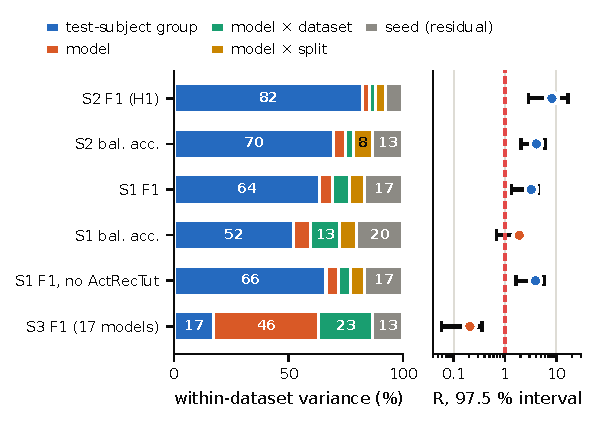
\includegraphics[width=\columnwidth]{figures/fig01_variance_components.pdf}
\caption{Where the within-dataset variance of the stored runs lies. Left: shares by source (numbers in \%). Right:
$R$ with its 97.5\,\% bootstrap interval; the dashed line is the pre-registered threshold. $R$ exceeds 1 in every
analysis of the shared-skeleton networks (on S1 with balanced accuracy its interval includes 1), and the network
dominates across the 17 heterogeneous published architectures (S3, conservative $R'$).}
\label{fig:vc}
\end{figure}

\begin{table}[t]
\caption{Variance components (F1 points$^2$) and $R$ [97.5\,\% interval]}
\label{tab:vc}
\centering
\setlength{\tabcolsep}{3pt}
\resizebox{\columnwidth}{!}{\begin{tabular}{@{}lrrrrrrl@{}}
\toprule
Analysis & $n$ & $\sigma^2_P$ & $\sigma^2_M$ & $\sigma^2_{MD}$ & $\sigma^2_{MP}$ & $\sigma^2_e$ & $R$ [97.5\,\% int.] \\
\midrule
S2 F1 (H1) & 828 & 127.7 & 4.8 & 4.0 & 6.9 & 11.7 & 8.19 [2.85, 16.90] \\
S2 bal. acc. & 828 & 86.3 & 6.5 & 4.4 & 10.1 & 16.6 & 4.09 [2.05, 6.03] \\
S1 F1 & 2160 & 66.2 & 5.9 & 7.8 & 6.7 & 17.6 & 3.26 [1.34, 4.47] \\
S1 bal. acc. & 2160 & 39.2 & 5.5 & 9.6 & 5.5 & 15.3 & 1.89 [0.69, 2.29] \\
S1 F1, no ActRecTut & 2100 & 67.4 & 5.5 & 5.1 & 6.5 & 17.0 & 3.93 [1.63, 5.80] \\
S3 F1 (17 models) & 510 & 37.5 & 100.2 & 51.0 & -- & 29.2 & 0.21 [0.06, 0.36] \\
\bottomrule
\end{tabular}
}
\end{table}

\subsection{Sensitivity analyses}
Balanced accuracy, which averages recall over the classes present and so has no per-split ceiling, gives
$R=\val{sens1_S2_balanced_accuracy.R}$ [\val{sens1_S2_balanced_accuracy.R_lo}, \val{sens1_S2_balanced_accuracy.R_hi}]
on S2: ceilings enlarge the subject share but do not create it. On the development set S1 the ordering is the same
with macro-F1 ($R=\val{sens2_S1_macro_f1.R}$ [\val{sens2_S1_macro_f1.R_lo}, \val{sens2_S1_macro_f1.R_hi}]), also
without its two-subject dataset ActRecTut ($R=\val{sens3_S1_without_actrectut.R}$); with balanced accuracy the point
estimate stays above 1 but the interval does not exclude it ($R=\val{sens2_S1_balanced_accuracy.R}$
[\val{sens2_S1_balanced_accuracy.R_lo}, \val{sens2_S1_balanced_accuracy.R_hi}]). Across the benchmark's 17 published architectures
it reverses: $R'=\val{sens4_S3_macro_f1.R}$ [\val{sens4_S3_macro_f1.R_lo}, \val{sens4_S3_macro_f1.R_hi}], with
$\sigma^2_M=\val{sens4_S3_macro_f1.s2_M}$ against $\sigma^2_P=\val{sens4_S3_macro_f1.s2_P}$. These architectures range
from k-NN to attention networks; their differences are far larger than those between the shared-skeleton networks.

\begin{figure}[t]
\centering
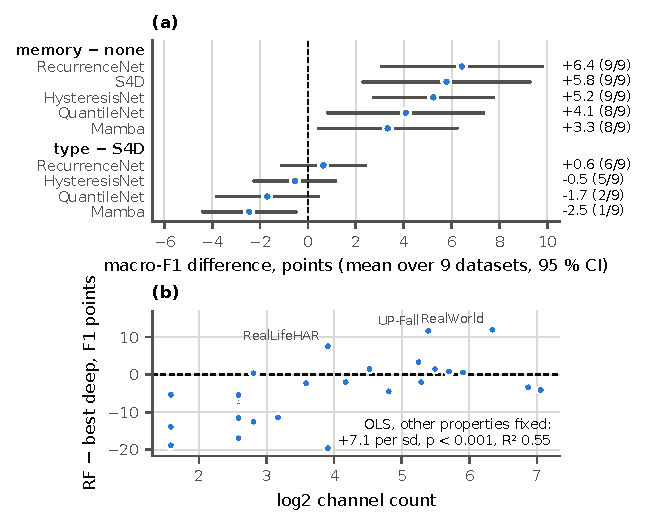
\includegraphics[width=\columnwidth]{figures/fig02_contrasts_channels.pdf}
\caption{Exploratory. (a) Temporal memory against none, and memory types against S4D, over the development datasets
whose runs pair by subject (mean and 95\,\% CI; datasets won). (b) Over the benchmark's 30 datasets (published single
runs), the Random Forest's margin over the best deep network rises with the number of sensor channels.}
\label{fig:explore}
\end{figure}

\subsection{Exploratory findings}
Within S1, the one design choice worth several points is temporal memory (Fig.~\ref{fig:explore}a): S4D gains
$\val{contrast.s4d-hystnet_nomem.9.mean}$ [$\val{contrast.s4d-hystnet_nomem.9.lo}$,
$\val{contrast.s4d-hystnet_nomem.9.hi}$] points over the same network without memory
(\val{contrast.s4d-hystnet_nomem.9.wins} of 9 datasets), while the type of memory moves macro-F1 by at most a few
points (Mamba $-$ S4D: $\val{contrast.mamba-s4d.9.mean}$ [$\val{contrast.mamba-s4d.9.lo}$,
$\val{contrast.mamba-s4d.9.hi}$]). Over the 30 datasets, a larger channel count goes with a larger margin of the
feature-based Random Forest over the best deep network ($\val{ols.rf.channels.beta}$ points per standard deviation of
$\log_2$ channels, $p\val{ols.rf.channels.p}$, other properties held fixed; Fig.~\ref{fig:explore}b), and fewer
training subjects go with a larger gap between the best and the median deep network
($\val{ols.gap.subjects.beta}$ per standard deviation, $p\val{ols.gap.subjects.p}$). No property predicts how hard a
dataset is ($R^2=\val{ols.level.r2}$).

\section{Discussion and Limitations}
For comparable networks, the subjects a wearable study records decide more of its macro-F1 than the network does:
the network-related variance on S2 is a fraction of the variance between test-subject groups, and a single seed adds
noise of its own. A comparison between such networks therefore needs many subjects, paired evaluation on the same
splits, several seeds, and a report of the spread across test subjects; a mean over a few splits cannot carry a gain
of one or two points. The reversal on S3 bounds the claim: a weak baseline is told apart from a strong network
easily, and the subject effect matters for choosing between designs that are already competitive. The exploratory
associations point at the sensing system: with many channels, hand-crafted features stay competitive, and with few
recorded subjects the choice of network matters more.

The analysis covers one protocol, and three seeds per run. The S1 and S2 networks share one skeleton, so their
components are controlled but not independent designs; S2's means were known before the registration; the
30-dataset results re-analyse published single runs and are correlational, and subjects and channels co-vary across
datasets. Re-execution covered the datasets cached on our cluster; the remaining runs are verified by their records.

\section{Conclusion}
Under a fixed person-disjoint protocol, who is tested accounts for most of the variance of macro-F1 among comparable
wearable HAR networks, as a pre-registered test on held-out datasets confirmed; across heterogeneous architectures
the network dominates. Studies of wearable sensing systems should size and report their test subjects accordingly.

\bibliographystyle{IEEEtran}
\bibliography{references}

\end{document}
